\documentclass[a4paper,12pt]{report}

\usepackage[utf8x]{inputenc}
\usepackage[T2A]{fontenc}
\usepackage[english, russian]{babel}

% Опционно, требует  apt-get install scalable-cyrfonts.*
% и удаления одной строчки в cyrtimes.sty
% Сточку не удалять!
% \usepackage{cyrtimes}

% Картнки и tikz
\usepackage{graphicx}
\usepackage{tikz}
\usetikzlibrary{snakes,arrows,shapes}


% Увы, поля придётся уменьшить из-за листингов.
\topmargin -1cm
\oddsidemargin -0.5cm
\evensidemargin -0.5cm
\textwidth 17cm
\textheight 24cm

\sloppy



% Оглавление в PDF
\usepackage[
bookmarks=true,
colorlinks=true, linkcolor=black, anchorcolor=black, citecolor=black, menucolor=black,filecolor=black, urlcolor=black,
unicode=true
]{hyperref}

% Для исходного кода в тексте
% \newcommand{\Code}[1]{\texttt{#1}}

% Некоторая русификация.
% \usepackage{misccorr} % Oh shi^W^W, оно не работает с report.
\usepackage{indentfirst}
\renewcommand{\labelitemi}{\normalfont\bfseries{--}}

% На дворе XXI век, но пакет listings всё ещё не пашет с русскими комментариями!

% Пакет listings для простой вставки исходников
% \usepackage{listings}
% Параметры оформления
% \lstset{
% showspaces=false,
% showtabs=false,
% frame=single,
% tabsize=4,
% basicstyle=\ttfamily,
% identifierstyle=\ttfamily,
% commentstyle=\itshape,
% stringstyle=\ttfamily,
% keywordstyle=\ttfamily,
% breaklines=true
% }
% Русский в комментариях.
% \lstset{escapebegin=\begin{cyr},escapeend=\end{cyr}}



% А это взято из файла, сгенерённого doxygen
\usepackage{calc}
\usepackage{array}
\newenvironment{Code}
{\footnotesize}
{\normalsize}
\newcommand{\doxyref}[3]{\textbf{#1} (\textnormal{#2}\,\pageref{#3})}
\newenvironment{DocInclude}
{\footnotesize}
{\normalsize}
\newenvironment{VerbInclude}
{\footnotesize}
{\normalsize}
\newenvironment{Image}
{\begin{figure}[H]}
{\end{figure}}
\newenvironment{ImageNoCaption}{}{}
\newenvironment{CompactList}
{\begin{list}{}{
  \setlength{\leftmargin}{0.5cm}
  \setlength{\itemsep}{0pt}
  \setlength{\parsep}{0pt}
  \setlength{\topsep}{0pt}
  \renewcommand{\makelabel}{\hfill}}}
{\end{list}}
\newenvironment{CompactItemize}
{
  \begin{itemize}
  \setlength{\itemsep}{-3pt}
  \setlength{\parsep}{0pt}
  \setlength{\topsep}{0pt}
  \setlength{\partopsep}{0pt}
}
{\end{itemize}}
\newcommand{\PBS}[1]{\let\temp=\\#1\let\\=\temp}
\newlength{\tmplength}
\newenvironment{TabularC}[1]
{
\setlength{\tmplength}
     {\linewidth/(#1)-\tabcolsep*2-\arrayrulewidth*(#1+1)/(#1)}
      \par\begin{tabular*}{\linewidth}
             {*{#1}{|>{\PBS\raggedright\hspace{0pt}}p{\the\tmplength}}|}
}
{\end{tabular*}\par}
\newcommand{\entrylabel}[1]{
   {\parbox[b]{\labelwidth-4pt}{\makebox[0pt][l]{\textbf{#1}}\vspace{1.5\baselineskip}}}}
\newenvironment{Desc}
{\begin{list}{}
  {
    \settowidth{\labelwidth}{40pt}
    \setlength{\leftmargin}{\labelwidth}
    \setlength{\parsep}{0pt}
    \setlength{\itemsep}{-4pt}
    \renewcommand{\makelabel}{\entrylabel}
  }
}
{\end{list}}
\newenvironment{Indent}
  {\begin{list}{}{\setlength{\leftmargin}{0.5cm}}
      \item[]\ignorespaces}
  {\unskip\end{list}}

\makeatletter
\renewcommand{\thesection}{%
  \ifnum\c@chapter<1 \@arabic\c@section
  \else \thechapter.\@arabic\c@section
  \fi
}
\makeatother

\title{РПЗ ПВС}
\author{Ершов Константин ИУ7-37}

\begin{document}

\maketitle

\tableofcontents
\newpage
\section{ВВЕДЕНИЕ}

\subsection{Задание на курсовую работу}
В рамках задания к курсовой работе по курсу "Протоколы вычислительных сетей" реализовать SMTP-клиент для отправки сообщений электронной почты. Вариант задания - \number21 подрузамевает использование вызова poll(), для организации обработки множества входящих соединений в размках одного процесса, и рабочих процессов. Также необходимо предусмотреть возможность ведения журнала работы программы. Журналирование должно быть реализованно в отдельном процессе.
\subsection{Цель и задачи работы} 
Целью данной курсовой работы является разработка SMTP-клиента для отправки сообщений электронной почты.

Задачи работы представлены ниже:
\begin{itemize}
	\itemСоздание SMTP-клиента (как части MTA), обеспечивающего удаленную доставку и поддерживающего очереди сообщений.

	\item Все варианты предполагают обработку нескольких исходящих соединений в одном потоке выполнения (т.е., одном процесс или одном потоке).

	\item На один удалённый MX надо создавать не более одного сокета (допустимый вариант — на один удалённый IP не более одного сокета).

	\item Следует использовать отдельную очередь собщений для каждого MX.		

\end{itemize}

\newpage
\section{АНАЛИТИЧЕСКИЙ РАЗДЕЛ}
В данном разделе представлено описание предметной области, выделены сущности предметной области, представлен способ разделения нагрузки между рабочими процессами.

\subsection{Предметная область}
В соответствии с выданным вариантом, необходимо реализовать SMTP-сервер для получения сообщений электронной почты с использованием poll() и рабочих процессов.

Поскольку обычно ввод-вывод осуществляется с использованием блокирующих системных вывозов, то при попытке считывания или записи данных программа будет блокироваться на этой операции и ожидать появления некоторых данных. Если программа производит работу над локальным файлом, то блокировка, обычно, не занимает долго времени. Однако при использовании сетевых сокетов, когда программа использует вызовы accept(), recv(), write() ожидание данных может занимать продолжительное время, поскольку возможна работа в условиях медленного соединения.

Для решения описанной выше проблемы возможно использование вызова poll(). При использовании poll() регистрируются множества файловых дескрипторов ожидающих записи или чтения. Когда появляется возможность записи или чтения в отслеживаемом дескрипторе, программа может выполнить требуемую операцию, проверив состояние дескриптора в соответствующем множестве.

Использование poll() позволяет производить обработку нескольких активных соединений в рамках одного процесса, и особенно эффективено при небольшом числе одновременно активных сокетов (передача в ядро и обратно по три байта на сокет). Также poll() выл портирован на множество различных ОС, что позволяет использовать его в переносимых программах. 

Ограничением работы с poll() являются максимальное количество отслеживаемых файловых дескрипторов равное 1024 (Linux). В некоторых ОС возможно увеличение этого значения изменив параметр FD\_SETSIZE, однако если необходима высокая переносимость программы, то этого значения может не хватать.

Получение и обработка запросов выполняется в рабочих процессах программы. Каждый процесс обрабатывает новые подключения, принимает и отправляет сообщения клиентам.

Многопроцессный подход к организации обработки сетевых соединений имеет неколько преимуществ перед однопроцессным, т.к. возникновение сбоев в работе одного процесса не приводит к завершению всей программы. При наличии реализации однопроцессной программы с FSM архитектурой, перевод ее на работу с несколькими процессами достаточно прост. Также с увеличением числа процессоров такие программы хорошо масштабируются. С использованием FSM архитектуры логики обработки заявок такой подход может быть высокоэффективным. Однако в некоторых ОС (Solaris, HP\_UX), где обработка потока программы производится быстрее процесса, эффективнее было бы использование потоков, вместо процессов. 

\subsection{Сущности предметной области}
Необходимо выделить основные сущности указанной предметной области. К ним относятся:

\begin{itemize}
	
		\item \textbf{Почтовый клиент} – отправитель письма. Им может выступать как почтовый клиент пользователя, так и другой SMTP-сервер. Имеет адрес, с которого устанавливается соединение с сервером. Отправитель формирует письмо и отправляет его на SMTP-сервер;
		\item \textbf{Письмо} – сообщение, передаваемое отправителем SMTP-серверу. Содержит поля TO - адрес получателя, FROM - адрес отправителя и текст письма. Письмо формируется отправителем и поступает на SMTP-сервер; 
		\item \textbf{SMTP-сервер} – сервер, получающий письма от отправителей. Имеет атрибуты: адрес сервера и порт. Служит для получения писем от отправителей; 

\end{itemize}

\newpage
В этой системе можно выделить следующие субъекты и соответствующие им прецеденты:

\textbf{SMTP-сервер} - инициирует один из прецедентов: получение данных письма, создание файла копии письма, завершение соединения.

Прецеденты:
\begin{itemize}
	
		\item \textbf{Получение данных письма} – при установлении подключения соединения к SMTP-серверу, клиент производит отправку данных письма(или нескольких писем в рамках одной сессии): данные об отправителе, получателе (или нескольких получателях), текст письма. В ответ на передаваемые серверу команды, он отправляет сообщения о результатах выполнения;
		\item \textbf{Создание файла копии письма} – после получения всех необходимых данных письма, SMTP-сервер осуществляет создание файла письма, который в дальнейшем используется SMTP-клиентом для пересылки почты. Данный прецедент может включать создание директорий пользователя, при проведенной ранее аутентификации;
		\item \textbf{Завершение соединения} – В случае возникновения ошибок в обмене сообщениями с клиентом, или по завершению обмена, SMTP-сервер разрывает соединение с клиентом, отправляя сообщение о разрыве соединения.

\end{itemize}

\subsection{Разделение нагрузки между рабочими процессами}

При разработке сервера с использованием нескольких рабочих процессов возникает задача распределения нагрузки по обработке входящих соединений между ними. 

В данной работе было предложено равномерное распределение нагрузки между рабочими процессами. При установке нового подключения его обработкой должен заниматься тот процесс, который обрабатывает наименьшее число активных соединений. Такой подход обеспечит равномерное распределение обработки соединений между рабочими процессами.

Алгоритм распределения нагрузки между рабочими процессами представлен следующим образом:

\begin{itemize}
	
		\item При инициализации программы главным процессом создается указанное число рабочих процессов;
		\item Каждому процессу назнается его ID - уникальный идентификатор. Главный процесс имеет ID = 0, рабочие процессы ID = 1,2,3... по порядку;
		\item Создается массив, хранящий текущее количество активных соединений каждого рабочего процесса. Начальное значение каждого элемента массива равно нулю;
		\item Объявляется переменная nproc, хранящая ID рабочего процесса, который должен обрабатывать новое подключениею. Начальное значение равно единице; 
		\item Главный процесс, используя массив количества активных подключений, выбирает рабочий процесс с наименьшим числом активных подключений и записывает его ID в переменную nproc;
		\item При установлении нового подключения, его обработкой займется процесс с ID = nproc. В момент установления нового подключения он увеличивает на единицу счетчик активных подключений;
		\item При разрыве соединения, или завершении цикла получения письма от получателя счетчик активных подключений уменьшается на единицу;			
		\item Три описанные выше шага поворяются до момента завершения работы программы.

\end{itemize}

Возможно возникновение ситуации, когда один из рабочих процессов был аварийно завершен (в случае возникновения в нем ошибок). Главный процесс, считывая массив активных подключений рабочих процессов, не зная о завершении процесса, будет назначать его кандидатом на обработку нового подключения. В данной ситуации такое поведение ошибочно и будет приводить к задержкам обработки или даже невозможности установления новых подключений. Для избежания этого была предусмотрена логика проверки состояния рабочего процесса с использованием вызова kill(2) перед изменением переменной nproc.


\section{Конструкторский раздел}

\subsection{Конечный автомат состояний клиента}

Процессы работы SMTP-сервера представлены в виде конечного автомата на Рис.~\ref{fig:fsm}, который описан в файле client.def.

\begin{figure}
\centering
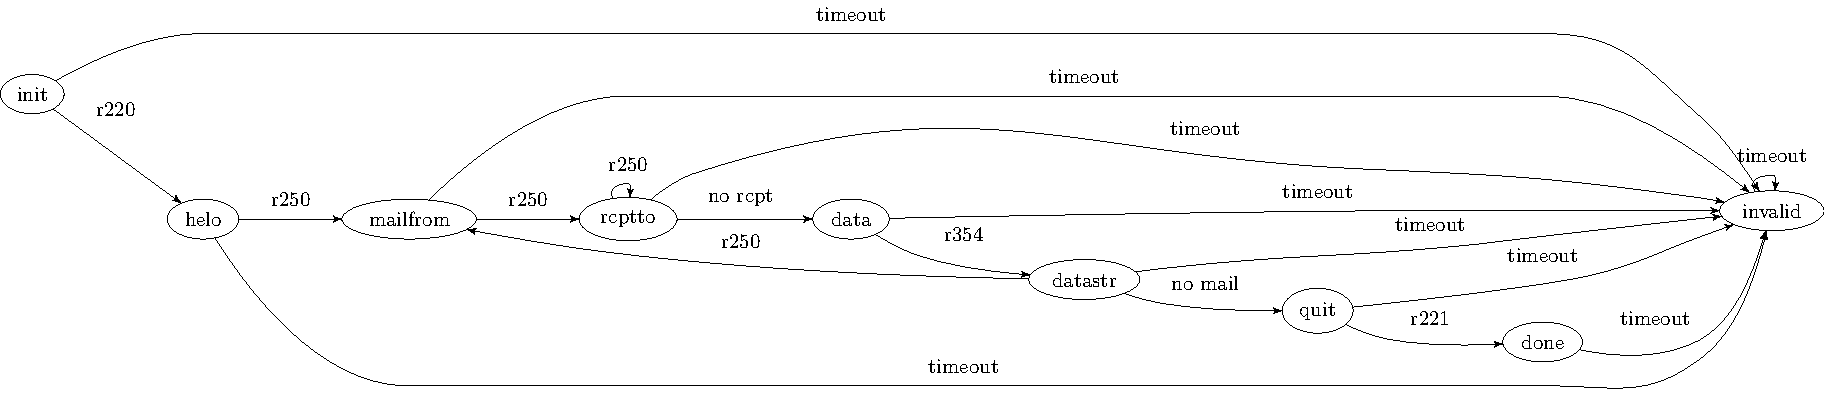
\includegraphics[width=\textwidth]{include/client_def_dot.pdf}
\caption{Состояния сервера}
\label{fig:fsm}
\end{figure}

\subsection{Синтаксис команд протокола}

\begin{description}
\item[220]
\texttt{\^{}220?:\textbackslash{}s+.+?\textbackslash{}r\textbackslash{}n}
\item[221]
\texttt{\^{}221?:\textbackslash{}s+.+?\textbackslash{}r\textbackslash{}n}
\item[250]
\texttt{\^{}250?:\textbackslash{}s+.+?\textbackslash{}r\textbackslash{}n}
\item[354]
\texttt{\^{}354?:\textbackslash{}s+.+?\textbackslash{}r\textbackslash{}n}
\item[data]
\texttt{\^{}DATA\textbackslash{}r\textbackslash{}n}
\item[mail from]
\texttt{\^{}MAIL FROM:\textbackslash{}s*<.+>\textbackslash{}r\textbackslash{}n}
\item[rcpt to]
\texttt{\^{}RCPT TO:\textbackslash{}s*<.+@.+>\textbackslash{}r\textbackslash{}n}
\item[mx dns]
\texttt{MX\textbackslash{}s+\textbackslash{}d+\textbackslash{}s*.+\.\$}
\end{description}

% \input{include/checkoptn.def.tex}
% \lstset{language=C}
% \lstinputlisting{../src/checkoptn.def}

\section{Технологический раздел}

\subsection{Сборка программы}

Сборка программы описана в файле \textit{Makefile} системы сборки \textit{make}. Рис.~\ref{fig:make} нагенерили самодельные \textit{makesimple} и \textit{makefile2dot}, а также \textit{dot2tex} и \textit{dot}.

\begin{figure}
\centering
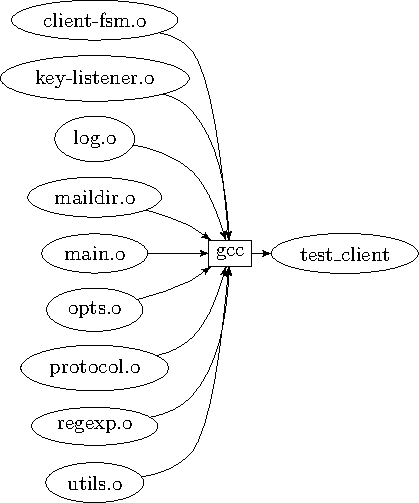
\includegraphics[width=\textwidth]{include/Makefile_1_dot.pdf}
\caption{Сборка программы}
\label{fig:make}
\end{figure}

Отмечу, что за исключения целей типа \textit{all}, \textit{install}, \textit{clean}, \textit{tests}, все имена целей в файле систем сборки \textit{make} обычно совпадают с именами файлов (такой вот низкоуровневый инструмент). То есть вместо цели \textit{lexer} следует использовать цель \textit{src/lexer.c}.

\subsection{Основные функции программы}

Весь это раздел сгеренерировал doxygen из части комментированных исходников программы. В файле конфигурации \textbf{doxyggen.cfg} был отключён параметр \textbf{HAVE\_DOT}, поскольку для рисования графов вызовов используется \textit{cflow}.

% \subsection{Файлы}
Полный список документированных файлов.\begin{DoxyCompactList}
\item\contentsline{section}{include/{\bfseries client-\/fsm.\-h} }{\pageref{client-fsm_8h}}{}
\item\contentsline{section}{include/\hyperlink{key-listener_8h}{key-\/listener.\-h} \\*Ожидание сигнала для завершения программы }{\pageref{key-listener_8h}}{}
\item\contentsline{section}{include/\hyperlink{log_8h}{log.\-h} \\*Логирование сообщений в отдельном процессе }{\pageref{log_8h}}{}
\item\contentsline{section}{include/\hyperlink{maildir_8h}{maildir.\-h} \\*Файл со структурами и функциями для работы с сообщениями }{\pageref{maildir_8h}}{}
\item\contentsline{section}{include/{\bfseries opts.\-h} }{\pageref{opts_8h}}{}
\item\contentsline{section}{include/\hyperlink{protocol_8h}{protocol.\-h} \\*Файл содержащий структуры и функции для работы по протоколу S\-M\-T\-P }{\pageref{protocol_8h}}{}
\item\contentsline{section}{include/{\bfseries queue.\-h} }{\pageref{queue_8h}}{}
\item\contentsline{section}{include/\hyperlink{regexp_8h}{regexp.\-h} \\*Набор функций для работы с регулярными выражениями. smtp\-\_\-re\-\_\-name перечисляет все представленные регулярные выражения }{\pageref{regexp_8h}}{}
\item\contentsline{section}{include/{\bfseries tree.\-h} }{\pageref{tree_8h}}{}
\item\contentsline{section}{include/{\bfseries utils.\-h} }{\pageref{utils_8h}}{}
\item\contentsline{section}{src/\hyperlink{key-listener_8c}{key-\/listener.\-c} \\*Функции и переменные для разбора команд }{\pageref{key-listener_8c}}{}
\item\contentsline{section}{src/\hyperlink{log_8c}{log.\-c} \\*Логирование сообщений в отдельном процессе }{\pageref{log_8c}}{}
\item\contentsline{section}{src/\hyperlink{maildir_8c}{maildir.\-c} \\*Файл со структурами и функциями для работы с сообщениями }{\pageref{maildir_8c}}{}
\item\contentsline{section}{src/\hyperlink{protocol_8c}{protocol.\-c} \\*Файл содержащий структуры и функции для работы по протоколу S\-M\-T\-P }{\pageref{protocol_8c}}{}
\item\contentsline{section}{src/\hyperlink{regexp_8c}{regexp.\-c} }{\pageref{regexp_8c}}{}
\end{DoxyCompactList}


\hypertarget{key-listener_8h}{\subsection{Файл include/key-\/listener.h}
\label{key-listener_8h}\index{include/key-\/listener.\-h@{include/key-\/listener.\-h}}
}


Ожидание сигнала для завершения программы  


\subsubsection*{Функции}
\begin{DoxyCompactItemize}
\item 
\hypertarget{key-listener_8h_afce84267d242a67489ca201c43c8cae6}{int {\bfseries keyboard\-\_\-listener\-\_\-fork} ()}\label{key-listener_8h_afce84267d242a67489ca201c43c8cae6}

\item 
\hypertarget{key-listener_8h_a0542378d05d3c52577c6f23db16bea6b}{int {\bfseries keyboard\-\_\-listener\-\_\-final} ()}\label{key-listener_8h_a0542378d05d3c52577c6f23db16bea6b}

\item 
\hypertarget{key-listener_8h_a25d43c3904f4a26b458c753fd7d83c26}{int {\bfseries quit\-\_\-key\-\_\-pressed} ()}\label{key-listener_8h_a25d43c3904f4a26b458c753fd7d83c26}

\end{DoxyCompactItemize}


\subsubsection{Подробное описание}
Ожидание сигнала для завершения программы Ожидание символа 'Q' ведется в отдельном потоке. При нажатии на эту клавишу основному процессу посылается сингла о том, что выполнение программы пора прекратить. Проверка на завершение следует производить через вызов функции quit\-\_\-key\-\_\-pressed(). 
\hypertarget{key-listener_8c}{\subsection{Файл src/key-\/listener.c}
\label{key-listener_8c}\index{src/key-\/listener.\-c@{src/key-\/listener.\-c}}
}


Функции и переменные для разбора команд.  


\subsubsection*{Функции}
\begin{DoxyCompactItemize}
\item 
\hypertarget{key-listener_8c_a83385f91069b8e1949d0360674ad3240}{int {\bfseries keyboard\-\_\-loop} ()}\label{key-listener_8c_a83385f91069b8e1949d0360674ad3240}

\item 
\hypertarget{key-listener_8c_afce84267d242a67489ca201c43c8cae6}{int {\bfseries keyboard\-\_\-listener\-\_\-fork} ()}\label{key-listener_8c_afce84267d242a67489ca201c43c8cae6}

\item 
\hypertarget{key-listener_8c_a25d43c3904f4a26b458c753fd7d83c26}{int {\bfseries quit\-\_\-key\-\_\-pressed} ()}\label{key-listener_8c_a25d43c3904f4a26b458c753fd7d83c26}

\item 
\hypertarget{key-listener_8c_a0542378d05d3c52577c6f23db16bea6b}{int {\bfseries keyboard\-\_\-listener\-\_\-final} ()}\label{key-listener_8c_a0542378d05d3c52577c6f23db16bea6b}

\end{DoxyCompactItemize}
\subsubsection*{Переменные}
\begin{DoxyCompactItemize}
\item 
\hypertarget{key-listener_8c_ac4a5c4cd6cd657b224681ccdb051bee7}{int \hyperlink{key-listener_8c_ac4a5c4cd6cd657b224681ccdb051bee7}{key\-\_\-sock}}\label{key-listener_8c_ac4a5c4cd6cd657b224681ccdb051bee7}

\begin{DoxyCompactList}\small\item\em Socket to pass exit signal. \end{DoxyCompactList}\end{DoxyCompactItemize}


\subsubsection{Подробное описание}
Функции и переменные для разбора команд. В этом файле описаны функции необходимые для работы key listener 
\hypertarget{log_8h}{\subsection{Файл include/log.h}
\label{log_8h}\index{include/log.\-h@{include/log.\-h}}
}


Логирование сообщений в отдельном процессе.  


\subsubsection*{Функции}
\begin{DoxyCompactItemize}
\item 
\hypertarget{log_8h_a850583634650fd49a0a948ad865ee5de}{int {\bfseries fork\-\_\-log} ()}\label{log_8h_a850583634650fd49a0a948ad865ee5de}

\item 
int \hyperlink{log_8h_afd4cbd54138e6ecd2035d8daf2ae1f2f}{close\-\_\-log} ()
\item 
\hypertarget{log_8h_a0ec50d6f386ce634b6269afb7cafc47c}{int {\bfseries send\-\_\-log} (char $\ast$msg)}\label{log_8h_a0ec50d6f386ce634b6269afb7cafc47c}

\end{DoxyCompactItemize}


\subsubsection{Подробное описание}
Логирование сообщений в отдельном процессе. Передача сообщений ведется через пару сокетов. Возможна раскраска сообщений. Три вида сообщений\-: отладка, ошибки, обычные.

Есть возможность включения/выключения режима отладки (пропадают все сообщения типа D\-L\-O\-G), работы лога в отдельном процессе (в таком случае все сообщения выводятся сразу же) и раскраски (все цвета не выводятся).

Ограничения\-: 1) первый аргумент любого макроса -\/ строка вида \char`\"{}...\char`\"{}; использование переменных в качестве первого параметра недопустимо; 2) максимальная длина сообщения установлена как M\-A\-X\-\_\-\-L\-O\-G\-\_\-\-M\-E\-S\-S\-A\-G\-E\-\_\-\-S\-I\-Z\-E; 3) для запуска лога следует использовать функцию fork\-\_\-log(), а для завершения -\/ \hyperlink{log_8h_afd4cbd54138e6ecd2035d8daf2ae1f2f}{close\-\_\-log()}; при этом основной процесс будет ожидать, пока не будут выведены все накопленные сообщения. 4) для логирования следует использовать макросы E\-L\-O\-G, D\-L\-O\-G и L\-O\-G; использование функции send\-\_\-log() недопустимо.





\subsubsection{Функции}
\hypertarget{log_8h_afd4cbd54138e6ecd2035d8daf2ae1f2f}{\index{log.\-h@{log.\-h}!close\-\_\-log@{close\-\_\-log}}
\index{close\-\_\-log@{close\-\_\-log}!log.h@{log.\-h}}
\paragraph[{close\-\_\-log}]{\setlength{\rightskip}{0pt plus 5cm}int close\-\_\-log (
\begin{DoxyParamCaption}
{}
\end{DoxyParamCaption}
)}}\label{log_8h_afd4cbd54138e6ecd2035d8daf2ae1f2f}
Send stop signal to log from main process and wait till log process finishes his work; if log is not forked, function just returns 
\hypertarget{log_8c}{\subsection{Файл src/log.c}
\label{log_8c}\index{src/log.\-c@{src/log.\-c}}
}


Логирование сообщений в отдельном процессе.  


\subsubsection*{Функции}
\begin{DoxyCompactItemize}
\item 
\hypertarget{log_8c_ad8f00388dc89407e5ab13d2380aa7a26}{int {\bfseries log\-\_\-message} (const char $\ast$buf, char type)}\label{log_8c_ad8f00388dc89407e5ab13d2380aa7a26}

\item 
\hypertarget{log_8c_a6e0151ead1f53b374b9e80ce4a40a476}{void {\bfseries log\-\_\-loop} ()}\label{log_8c_a6e0151ead1f53b374b9e80ce4a40a476}

\item 
\hypertarget{log_8c_a850583634650fd49a0a948ad865ee5de}{int {\bfseries fork\-\_\-log} ()}\label{log_8c_a850583634650fd49a0a948ad865ee5de}

\item 
int \hyperlink{log_8c_afd4cbd54138e6ecd2035d8daf2ae1f2f}{close\-\_\-log} ()
\item 
\hypertarget{log_8c_a0ec50d6f386ce634b6269afb7cafc47c}{int {\bfseries send\-\_\-log} (char $\ast$msg)}\label{log_8c_a0ec50d6f386ce634b6269afb7cafc47c}

\end{DoxyCompactItemize}
\subsubsection*{Переменные}
\begin{DoxyCompactItemize}
\item 
int \hyperlink{log_8c_a9e689815c90dafeed44e7088b718c8ea}{msg\-\_\-sock}
\end{DoxyCompactItemize}


\subsubsection{Подробное описание}
Логирование сообщений в отдельном процессе. Передача сообщений ведется через пару сокетов. Возможна раскраска сообщений. Три вида сообщений\-: отладка, ошибки, обычные. 

\subsubsection{Функции}
\hypertarget{log_8c_afd4cbd54138e6ecd2035d8daf2ae1f2f}{\index{log.\-c@{log.\-c}!close\-\_\-log@{close\-\_\-log}}
\index{close\-\_\-log@{close\-\_\-log}!log.c@{log.\-c}}
\paragraph[{close\-\_\-log}]{\setlength{\rightskip}{0pt plus 5cm}int close\-\_\-log (
\begin{DoxyParamCaption}
{}
\end{DoxyParamCaption}
)}}\label{log_8c_afd4cbd54138e6ecd2035d8daf2ae1f2f}
Send stop signal to log from main process and wait till log process finishes his work; if log is not forked, function just returns 

\subsubsection{Переменные}
\hypertarget{log_8c_a9e689815c90dafeed44e7088b718c8ea}{\index{log.\-c@{log.\-c}!msg\-\_\-sock@{msg\-\_\-sock}}
\index{msg\-\_\-sock@{msg\-\_\-sock}!log.c@{log.\-c}}
\paragraph[{msg\-\_\-sock}]{\setlength{\rightskip}{0pt plus 5cm}int msg\-\_\-sock}}\label{log_8c_a9e689815c90dafeed44e7088b718c8ea}
Socket\-: 1) to get messages (from log); 2) to send messages (from main process) 
\hypertarget{maildir_8h}{\subsection{Файл include/maildir.h}
\label{maildir_8h}\index{include/maildir.\-h@{include/maildir.\-h}}
}


Файл со структурами и функциями для работы с сообщениями  


\subsubsection*{Структуры данных}
\begin{DoxyCompactItemize}
\item 
struct \hyperlink{structrcpt}{rcpt}
\begin{DoxyCompactList}\small\item\em Структура для хранения имени и домена получателя \end{DoxyCompactList}\item 
struct \hyperlink{structmail}{mail}
\begin{DoxyCompactList}\small\item\em Структура для хранения писем \end{DoxyCompactList}\end{DoxyCompactItemize}
\subsubsection*{Перечисления}
\begin{DoxyCompactItemize}
\item 
enum {\bfseries maildir\-\_\-dir} \{ \\*
{\bfseries D\-I\-R\-\_\-\-R\-O\-O\-T}, 
{\bfseries D\-I\-R\-\_\-\-N\-E\-W}, 
{\bfseries D\-I\-R\-\_\-\-C\-U\-R}, 
{\bfseries D\-I\-R\-\_\-\-N\-O\-T\-S\-E\-N\-T}, 
\\*
{\bfseries maildir\-\_\-count}
 \}
\end{DoxyCompactItemize}
\subsubsection*{Функции}
\begin{DoxyCompactItemize}
\item 
\hypertarget{maildir_8h_abbd06722d933d8849bd940ed8056d8e0}{{\bfseries T\-A\-I\-L\-Q\-\_\-\-H\-E\-A\-D} (rcpt\-\_\-list, \hyperlink{structrcpt}{rcpt})}\label{maildir_8h_abbd06722d933d8849bd940ed8056d8e0}

\item 
\hypertarget{maildir_8h_a421f8811d7be9747f564badf4523a88c}{{\bfseries T\-A\-I\-L\-Q\-\_\-\-H\-E\-A\-D} (mail\-\_\-list, \hyperlink{structmail}{mail})}\label{maildir_8h_a421f8811d7be9747f564badf4523a88c}

\item 
\hypertarget{maildir_8h_a1e9cbe73bb98af1f8b67d4a428dbb1d3}{int {\bfseries maildir\-\_\-init} ()}\label{maildir_8h_a1e9cbe73bb98af1f8b67d4a428dbb1d3}

\item 
\hypertarget{maildir_8h_a5a714eaef0349162b8106f58dc8fa241}{int {\bfseries maildir\-\_\-final} ()}\label{maildir_8h_a5a714eaef0349162b8106f58dc8fa241}

\item 
\hypertarget{maildir_8h_aea5a119f35196c3ea74b9c7a9ec34056}{void {\bfseries free\-\_\-mail} (struct \hyperlink{structmail}{mail} $\ast$m)}\label{maildir_8h_aea5a119f35196c3ea74b9c7a9ec34056}

\item 
\hypertarget{maildir_8h_a8d846fd3a0e5f094a330c540e45493b3}{void {\bfseries free\-\_\-mail\-\_\-list} (struct mail\-\_\-list $\ast$ml)}\label{maildir_8h_a8d846fd3a0e5f094a330c540e45493b3}

\item 
\hypertarget{maildir_8h_aa63c3b5e1e9bd42357c62aa6e3b5b7bc}{int {\bfseries new\-\_\-mail\-\_\-exist} ()}\label{maildir_8h_aa63c3b5e1e9bd42357c62aa6e3b5b7bc}

\item 
\hypertarget{maildir_8h_afecf772b58de12e2a17167438eb988d5}{void {\bfseries move\-\_\-mail} (const char $\ast$filename, maildir\-\_\-dir from\-\_\-dir, maildir\-\_\-dir to\-\_\-dir)}\label{maildir_8h_afecf772b58de12e2a17167438eb988d5}

\item 
\hypertarget{maildir_8h_a25a46de8004b6c7eb1683230d60f53ce}{void {\bfseries copy\-\_\-mail} (const char $\ast$filename, maildir\-\_\-dir from\-\_\-dir, maildir\-\_\-dir to\-\_\-dir)}\label{maildir_8h_a25a46de8004b6c7eb1683230d60f53ce}

\item 
\hypertarget{maildir_8h_a400c412a291331a3564e5c8397a63cff}{void {\bfseries delete\-\_\-mail} (const char $\ast$filename, maildir\-\_\-dir dir)}\label{maildir_8h_a400c412a291331a3564e5c8397a63cff}

\item 
\hypertarget{maildir_8h_a6d909dab94890273728a5cc9966f9cb6}{int {\bfseries filter\-\_\-my\-\_\-mail} (struct mail\-\_\-list $\ast$ml)}\label{maildir_8h_a6d909dab94890273728a5cc9966f9cb6}

\item 
\hypertarget{maildir_8h_a33a565cf3328ab035bc1099c040f1292}{int {\bfseries read\-\_\-all\-\_\-mail} (struct mail\-\_\-list $\ast$ml)}\label{maildir_8h_a33a565cf3328ab035bc1099c040f1292}

\item 
\hypertarget{maildir_8h_a9bc971a3c04578afe451897ccbab946a}{struct \hyperlink{structmail}{mail} $\ast$ {\bfseries read\-\_\-mail\-\_\-file} (const char $\ast$filename)}\label{maildir_8h_a9bc971a3c04578afe451897ccbab946a}

\item 
\hypertarget{maildir_8h_a1e6e8ef62eb133f023d676889804bbca}{int {\bfseries read\-\_\-mail\-\_\-from} (F\-I\-L\-E $\ast$f, struct \hyperlink{structmail}{mail} $\ast$m)}\label{maildir_8h_a1e6e8ef62eb133f023d676889804bbca}

\item 
\hypertarget{maildir_8h_aefb5606408f4df2065991ac5dc8d03f5}{int {\bfseries read\-\_\-mail\-\_\-to} (F\-I\-L\-E $\ast$f, struct \hyperlink{structmail}{mail} $\ast$m)}\label{maildir_8h_aefb5606408f4df2065991ac5dc8d03f5}

\item 
\hypertarget{maildir_8h_a86c99727ccc6619cfe2b11a143ac0c53}{int {\bfseries read\-\_\-mail\-\_\-data} (F\-I\-L\-E $\ast$f, struct \hyperlink{structmail}{mail} $\ast$m)}\label{maildir_8h_a86c99727ccc6619cfe2b11a143ac0c53}

\end{DoxyCompactItemize}


\subsubsection{Подробное описание}
Файл со структурами и функциями для работы с сообщениями 
\hypertarget{maildir_8c}{\subsection{Файл src/maildir.c}
\label{maildir_8c}\index{src/maildir.\-c@{src/maildir.\-c}}
}


Файл со структурами и функциями для работы с сообщениями  


\subsubsection*{Функции}
\begin{DoxyCompactItemize}
\item 
\hypertarget{maildir_8c_a1e9cbe73bb98af1f8b67d4a428dbb1d3}{int {\bfseries maildir\-\_\-init} ()}\label{maildir_8c_a1e9cbe73bb98af1f8b67d4a428dbb1d3}

\item 
\hypertarget{maildir_8c_a5a714eaef0349162b8106f58dc8fa241}{int {\bfseries maildir\-\_\-final} ()}\label{maildir_8c_a5a714eaef0349162b8106f58dc8fa241}

\item 
\hypertarget{maildir_8c_aa63c3b5e1e9bd42357c62aa6e3b5b7bc}{int {\bfseries new\-\_\-mail\-\_\-exist} ()}\label{maildir_8c_aa63c3b5e1e9bd42357c62aa6e3b5b7bc}

\item 
\hypertarget{maildir_8c_a33a565cf3328ab035bc1099c040f1292}{int {\bfseries read\-\_\-all\-\_\-mail} (struct mail\-\_\-list $\ast$ml)}\label{maildir_8c_a33a565cf3328ab035bc1099c040f1292}

\item 
\hypertarget{maildir_8c_a9bc971a3c04578afe451897ccbab946a}{struct \hyperlink{structmail}{mail} $\ast$ {\bfseries read\-\_\-mail\-\_\-file} (const char $\ast$filename)}\label{maildir_8c_a9bc971a3c04578afe451897ccbab946a}

\item 
\hypertarget{maildir_8c_a1e6e8ef62eb133f023d676889804bbca}{int {\bfseries read\-\_\-mail\-\_\-from} (F\-I\-L\-E $\ast$f, struct \hyperlink{structmail}{mail} $\ast$m)}\label{maildir_8c_a1e6e8ef62eb133f023d676889804bbca}

\item 
\hypertarget{maildir_8c_aefb5606408f4df2065991ac5dc8d03f5}{int {\bfseries read\-\_\-mail\-\_\-to} (F\-I\-L\-E $\ast$f, struct \hyperlink{structmail}{mail} $\ast$m)}\label{maildir_8c_aefb5606408f4df2065991ac5dc8d03f5}

\item 
\hypertarget{maildir_8c_a86c99727ccc6619cfe2b11a143ac0c53}{int {\bfseries read\-\_\-mail\-\_\-data} (F\-I\-L\-E $\ast$f, struct \hyperlink{structmail}{mail} $\ast$m)}\label{maildir_8c_a86c99727ccc6619cfe2b11a143ac0c53}

\item 
\hypertarget{maildir_8c_a6d909dab94890273728a5cc9966f9cb6}{int {\bfseries filter\-\_\-my\-\_\-mail} (struct mail\-\_\-list $\ast$ml)}\label{maildir_8c_a6d909dab94890273728a5cc9966f9cb6}

\item 
\hypertarget{maildir_8c_aea5a119f35196c3ea74b9c7a9ec34056}{void {\bfseries free\-\_\-mail} (struct \hyperlink{structmail}{mail} $\ast$m)}\label{maildir_8c_aea5a119f35196c3ea74b9c7a9ec34056}

\item 
\hypertarget{maildir_8c_a8d846fd3a0e5f094a330c540e45493b3}{void {\bfseries free\-\_\-mail\-\_\-list} (struct mail\-\_\-list $\ast$ml)}\label{maildir_8c_a8d846fd3a0e5f094a330c540e45493b3}

\item 
\hypertarget{maildir_8c_afecf772b58de12e2a17167438eb988d5}{void {\bfseries move\-\_\-mail} (const char $\ast$filename, maildir\-\_\-dir from\-\_\-dir, maildir\-\_\-dir to\-\_\-dir)}\label{maildir_8c_afecf772b58de12e2a17167438eb988d5}

\item 
\hypertarget{maildir_8c_a25a46de8004b6c7eb1683230d60f53ce}{void {\bfseries copy\-\_\-mail} (const char $\ast$filename, maildir\-\_\-dir from\-\_\-dir, maildir\-\_\-dir to\-\_\-dir)}\label{maildir_8c_a25a46de8004b6c7eb1683230d60f53ce}

\item 
\hypertarget{maildir_8c_a400c412a291331a3564e5c8397a63cff}{void {\bfseries delete\-\_\-mail} (const char $\ast$filename, maildir\-\_\-dir dir)}\label{maildir_8c_a400c412a291331a3564e5c8397a63cff}

\end{DoxyCompactItemize}
\subsubsection*{Переменные}
\begin{DoxyCompactItemize}
\item 
\hypertarget{maildir_8c_a8bd6fbdf7f02b3a757954d25f01d315c}{char $\ast$ {\bfseries maildir\-\_\-path} \mbox{[}maildir\-\_\-count\mbox{]}}\label{maildir_8c_a8bd6fbdf7f02b3a757954d25f01d315c}

\end{DoxyCompactItemize}


\subsubsection{Подробное описание}
Файл со структурами и функциями для работы с сообщениями 
\hypertarget{protocol_8h}{\subsection{Файл include/protocol.h}
\label{protocol_8h}\index{include/protocol.\-h@{include/protocol.\-h}}
}


Файл содержащий структуры и функции для работы по протоколу S\-M\-T\-P.  


\subsubsection*{Структуры данных}
\begin{DoxyCompactItemize}
\item 
struct \hyperlink{structmx__conn}{mx\-\_\-conn}
\item 
struct \hyperlink{structdomain}{domain}
\end{DoxyCompactItemize}
\subsubsection*{Функции}
\begin{DoxyCompactItemize}
\item 
\hypertarget{protocol_8h_a6eee60cb94c7f9c2aa01785d478f2d5a}{{\bfseries T\-A\-I\-L\-Q\-\_\-\-H\-E\-A\-D} (mx\-\_\-conn\-\_\-list, \hyperlink{structmx__conn}{mx\-\_\-conn})}\label{protocol_8h_a6eee60cb94c7f9c2aa01785d478f2d5a}

\item 
\hypertarget{protocol_8h_a164d15a8b3fc169a08768a90d9ccf2b1}{{\bfseries T\-A\-I\-L\-Q\-\_\-\-H\-E\-A\-D} (domain\-\_\-set, \hyperlink{structdomain}{domain})}\label{protocol_8h_a164d15a8b3fc169a08768a90d9ccf2b1}

\item 
\hypertarget{protocol_8h_a21cc93a4b19d0b161ab7ddc0db847768}{int \hyperlink{protocol_8h_a21cc93a4b19d0b161ab7ddc0db847768}{smtp\-\_\-client\-\_\-loop} ()}\label{protocol_8h_a21cc93a4b19d0b161ab7ddc0db847768}

\begin{DoxyCompactList}\small\item\em Основная функция, которая мониторит директорию с почтой, чтобы ее отправить \end{DoxyCompactList}\item 
\hypertarget{protocol_8h_a9bd22b876331743b1b7ea35bc202ac3d}{int \hyperlink{protocol_8h_a9bd22b876331743b1b7ea35bc202ac3d}{conn\-\_\-init} ()}\label{protocol_8h_a9bd22b876331743b1b7ea35bc202ac3d}

\begin{DoxyCompactList}\small\item\em Initialize structures for connections with several S\-M\-T\-P servers. \end{DoxyCompactList}\item 
\hypertarget{protocol_8h_a79bd91966c052d0350da3af975e901f7}{void {\bfseries conn\-\_\-loop} ()}\label{protocol_8h_a79bd91966c052d0350da3af975e901f7}

\item 
\hypertarget{protocol_8h_ae6de6df669448d5fe834197125c63018}{int \hyperlink{protocol_8h_ae6de6df669448d5fe834197125c63018}{conn\-\_\-final} ()}\label{protocol_8h_ae6de6df669448d5fe834197125c63018}

\begin{DoxyCompactList}\small\item\em Frees all structures used in mail transfer. \end{DoxyCompactList}\item 
void \hyperlink{protocol_8h_a63b0324a5f0d042dab0ee3c372b73c2b}{domain\-\_\-add} (struct domain\-\_\-set $\ast$domains, char $\ast$new\-\_\-domain\-\_\-name)
\begin{DoxyCompactList}\small\item\em Adds another domain into domain set if it is not present there and if it is not local domain (M\-Y\-\_\-\-D\-O\-M\-A\-I\-N in \hyperlink{maildir_8h}{maildir.\-h}) \end{DoxyCompactList}\item 
\hypertarget{protocol_8h_a2678d96b53074a15c6b7ada9fd7e274b}{int {\bfseries rcpt\-\_\-is\-\_\-from\-\_\-domain} (struct \hyperlink{structrcpt}{rcpt} $\ast$r, struct \hyperlink{structdomain}{domain} $\ast$d)}\label{protocol_8h_a2678d96b53074a15c6b7ada9fd7e274b}

\item 
\hypertarget{protocol_8h_a3e6be25d869e115193d1b0d5cde9ad07}{int {\bfseries mail\-\_\-has\-\_\-rcpts\-\_\-from\-\_\-domain} (struct \hyperlink{structmail}{mail} $\ast$m, struct \hyperlink{structdomain}{domain} $\ast$d)}\label{protocol_8h_a3e6be25d869e115193d1b0d5cde9ad07}

\item 
\hypertarget{protocol_8h_a9ed99410a3642cb510821f00078e836c}{int {\bfseries check\-\_\-dns} (char $\ast$d, char $\ast$output\-\_\-address)}\label{protocol_8h_a9ed99410a3642cb510821f00078e836c}

\item 
\hypertarget{protocol_8h_a25299c3335401ec40597d96a2df0bcbc}{struct \hyperlink{structmx__conn}{mx\-\_\-conn} $\ast$ {\bfseries create\-\_\-connection} (struct \hyperlink{structdomain}{domain} $\ast$dom)}\label{protocol_8h_a25299c3335401ec40597d96a2df0bcbc}

\item 
\hypertarget{protocol_8h_a001371cf331cd6ea30938cf006b8d3da}{struct \hyperlink{structmx__conn}{mx\-\_\-conn} $\ast$ {\bfseries get\-\_\-conn\-\_\-by\-\_\-socket} (struct mx\-\_\-conn\-\_\-list $\ast$cl, int sock)}\label{protocol_8h_a001371cf331cd6ea30938cf006b8d3da}

\item 
\hypertarget{protocol_8h_a9c29bf6383c84c0b734d3b37144482cc}{int {\bfseries wait\-\_\-for\-\_\-response} ()}\label{protocol_8h_a9c29bf6383c84c0b734d3b37144482cc}

\item 
\hypertarget{protocol_8h_a65e032c3158ec7a8f167cd283cbef59c}{int {\bfseries parse\-\_\-response} (struct \hyperlink{structmx__conn}{mx\-\_\-conn} $\ast$conn, char $\ast$str, int length)}\label{protocol_8h_a65e032c3158ec7a8f167cd283cbef59c}

\item 
\hypertarget{protocol_8h_aafcf74851e51a77bff23afc1736df4b3}{void {\bfseries invalidate\-\_\-connection} (struct \hyperlink{structmx__conn}{mx\-\_\-conn} $\ast$conn)}\label{protocol_8h_aafcf74851e51a77bff23afc1736df4b3}

\item 
\hypertarget{protocol_8h_a6f3dd652b874d52d3ce7f2486540ce48}{int {\bfseries send\-\_\-hello} (struct \hyperlink{structmx__conn}{mx\-\_\-conn} $\ast$conn)}\label{protocol_8h_a6f3dd652b874d52d3ce7f2486540ce48}

\item 
\hypertarget{protocol_8h_a8b10f5e2dc31026fd53ca4754c9cceea}{int {\bfseries send\-\_\-mailfrom} (struct \hyperlink{structmx__conn}{mx\-\_\-conn} $\ast$conn)}\label{protocol_8h_a8b10f5e2dc31026fd53ca4754c9cceea}

\item 
\hypertarget{protocol_8h_a0f46c7536b8a12e73de1883b196696b5}{int {\bfseries send\-\_\-rcptto} (struct \hyperlink{structmx__conn}{mx\-\_\-conn} $\ast$conn)}\label{protocol_8h_a0f46c7536b8a12e73de1883b196696b5}

\item 
\hypertarget{protocol_8h_a7f08ff74d834d14d6aaf5b6d19b99085}{int {\bfseries send\-\_\-data} (struct \hyperlink{structmx__conn}{mx\-\_\-conn} $\ast$conn)}\label{protocol_8h_a7f08ff74d834d14d6aaf5b6d19b99085}

\item 
\hypertarget{protocol_8h_ac7ec4afbac17b4a2c788784dc68bad09}{int {\bfseries send\-\_\-datastr} (struct \hyperlink{structmx__conn}{mx\-\_\-conn} $\ast$conn)}\label{protocol_8h_ac7ec4afbac17b4a2c788784dc68bad09}

\item 
\hypertarget{protocol_8h_a248f9650f3fac8b3ac1d8f56f3a43822}{int {\bfseries send\-\_\-quit} (struct \hyperlink{structmx__conn}{mx\-\_\-conn} $\ast$conn)}\label{protocol_8h_a248f9650f3fac8b3ac1d8f56f3a43822}

\end{DoxyCompactItemize}


\subsubsection{Подробное описание}
Файл содержащий структуры и функции для работы по протоколу S\-M\-T\-P. 

\subsubsection{Функции}
\hypertarget{protocol_8h_a63b0324a5f0d042dab0ee3c372b73c2b}{\index{protocol.\-h@{protocol.\-h}!domain\-\_\-add@{domain\-\_\-add}}
\index{domain\-\_\-add@{domain\-\_\-add}!protocol.h@{protocol.\-h}}
\paragraph[{domain\-\_\-add}]{\setlength{\rightskip}{0pt plus 5cm}void domain\-\_\-add (
\begin{DoxyParamCaption}
\item[{struct domain\-\_\-set $\ast$}]{domains, }
\item[{char $\ast$}]{new\-\_\-domain\-\_\-name}
\end{DoxyParamCaption}
)}}\label{protocol_8h_a63b0324a5f0d042dab0ee3c372b73c2b}


Adds another domain into domain set if it is not present there and if it is not local domain (M\-Y\-\_\-\-D\-O\-M\-A\-I\-N in \hyperlink{maildir_8h}{maildir.\-h}) 


\begin{DoxyParams}{Аргументы}
{\em domains} & -- список доменов куда нужно добавить \\
\hline
{\em new\-\_\-domain\-\_\-name} & -- имя домена для добавления \\
\hline
\end{DoxyParams}

\hypertarget{protocol_8c}{\subsection{Файл src/protocol.c}
\label{protocol_8c}\index{src/protocol.\-c@{src/protocol.\-c}}
}


Файл содержащий структуры и функции для работы по протоколу S\-M\-T\-P.  


\subsubsection*{Функции}
\begin{DoxyCompactItemize}
\item 
\hypertarget{protocol_8c_a21cc93a4b19d0b161ab7ddc0db847768}{int \hyperlink{protocol_8c_a21cc93a4b19d0b161ab7ddc0db847768}{smtp\-\_\-client\-\_\-loop} ()}\label{protocol_8c_a21cc93a4b19d0b161ab7ddc0db847768}

\begin{DoxyCompactList}\small\item\em Основная функция, которая мониторит директорию с почтой, чтобы ее отправить \end{DoxyCompactList}\item 
\hypertarget{protocol_8c_a9bd22b876331743b1b7ea35bc202ac3d}{int \hyperlink{protocol_8c_a9bd22b876331743b1b7ea35bc202ac3d}{conn\-\_\-init} ()}\label{protocol_8c_a9bd22b876331743b1b7ea35bc202ac3d}

\begin{DoxyCompactList}\small\item\em Initialize structures for connections with several S\-M\-T\-P servers. \end{DoxyCompactList}\item 
\hypertarget{protocol_8c_a7c7fde4f333bb1f781b2a90eeb37d8e6}{int {\bfseries free\-\_\-connection} (struct \hyperlink{structmx__conn}{mx\-\_\-conn} $\ast$conn)}\label{protocol_8c_a7c7fde4f333bb1f781b2a90eeb37d8e6}

\item 
\hypertarget{protocol_8c_aa456fbb7e347e4f89e2453d4d3325cdf}{int {\bfseries free\-\_\-domain} (struct \hyperlink{structdomain}{domain} $\ast$d)}\label{protocol_8c_aa456fbb7e347e4f89e2453d4d3325cdf}

\item 
\hypertarget{protocol_8c_ae6de6df669448d5fe834197125c63018}{int \hyperlink{protocol_8c_ae6de6df669448d5fe834197125c63018}{conn\-\_\-final} ()}\label{protocol_8c_ae6de6df669448d5fe834197125c63018}

\begin{DoxyCompactList}\small\item\em Frees all structures used in mail transfer. \end{DoxyCompactList}\item 
void \hyperlink{protocol_8c_a7db98c4c210ef2fc7f86e5c01cd692ab}{domain\-\_\-add} (struct domain\-\_\-set $\ast$domains, char $\ast$new\-\_\-domain\-\_\-name)
\begin{DoxyCompactList}\small\item\em Adds another domain into domain set if it is not present there and if it is not local domain (M\-Y\-\_\-\-D\-O\-M\-A\-I\-N in \hyperlink{maildir_8h}{maildir.\-h}) \end{DoxyCompactList}\item 
\hypertarget{protocol_8c_a2678d96b53074a15c6b7ada9fd7e274b}{int {\bfseries rcpt\-\_\-is\-\_\-from\-\_\-domain} (struct \hyperlink{structrcpt}{rcpt} $\ast$r, struct \hyperlink{structdomain}{domain} $\ast$d)}\label{protocol_8c_a2678d96b53074a15c6b7ada9fd7e274b}

\item 
\hypertarget{protocol_8c_a3e6be25d869e115193d1b0d5cde9ad07}{int {\bfseries mail\-\_\-has\-\_\-rcpts\-\_\-from\-\_\-domain} (struct \hyperlink{structmail}{mail} $\ast$m, struct \hyperlink{structdomain}{domain} $\ast$d)}\label{protocol_8c_a3e6be25d869e115193d1b0d5cde9ad07}

\item 
\hypertarget{protocol_8c_a52d095a5c787424e1ac677c95f7d09f6}{int {\bfseries connect\-\_\-with\-\_\-timeout} (int sock, struct addrinfo $\ast$addr, int ms)}\label{protocol_8c_a52d095a5c787424e1ac677c95f7d09f6}

\item 
\hypertarget{protocol_8c_a7d17f0cebbce6bb33e6971fb50381de1}{int {\bfseries connect\-\_\-to\-\_\-any\-\_\-with\-\_\-timeout} (struct addrinfo $\ast$info, int ms)}\label{protocol_8c_a7d17f0cebbce6bb33e6971fb50381de1}

\item 
\hypertarget{protocol_8c_a25299c3335401ec40597d96a2df0bcbc}{struct \hyperlink{structmx__conn}{mx\-\_\-conn} $\ast$ {\bfseries create\-\_\-connection} (struct \hyperlink{structdomain}{domain} $\ast$dom)}\label{protocol_8c_a25299c3335401ec40597d96a2df0bcbc}

\item 
\hypertarget{protocol_8c_a9ed99410a3642cb510821f00078e836c}{int {\bfseries check\-\_\-dns} (char $\ast$d, char $\ast$output\-\_\-address)}\label{protocol_8c_a9ed99410a3642cb510821f00078e836c}

\item 
\hypertarget{protocol_8c_a001371cf331cd6ea30938cf006b8d3da}{struct \hyperlink{structmx__conn}{mx\-\_\-conn} $\ast$ {\bfseries get\-\_\-conn\-\_\-by\-\_\-socket} (struct mx\-\_\-conn\-\_\-list $\ast$cl, int sock)}\label{protocol_8c_a001371cf331cd6ea30938cf006b8d3da}

\item 
\hypertarget{protocol_8c_a79bd91966c052d0350da3af975e901f7}{void {\bfseries conn\-\_\-loop} ()}\label{protocol_8c_a79bd91966c052d0350da3af975e901f7}

\item 
\hypertarget{protocol_8c_a65e032c3158ec7a8f167cd283cbef59c}{int {\bfseries parse\-\_\-response} (struct \hyperlink{structmx__conn}{mx\-\_\-conn} $\ast$conn, char $\ast$str, int length)}\label{protocol_8c_a65e032c3158ec7a8f167cd283cbef59c}

\item 
\hypertarget{protocol_8c_aafcf74851e51a77bff23afc1736df4b3}{void {\bfseries invalidate\-\_\-connection} (struct \hyperlink{structmx__conn}{mx\-\_\-conn} $\ast$conn)}\label{protocol_8c_aafcf74851e51a77bff23afc1736df4b3}

\item 
\hypertarget{protocol_8c_a9c29bf6383c84c0b734d3b37144482cc}{int {\bfseries wait\-\_\-for\-\_\-response} ()}\label{protocol_8c_a9c29bf6383c84c0b734d3b37144482cc}

\item 
\hypertarget{protocol_8c_a6f3dd652b874d52d3ce7f2486540ce48}{int {\bfseries send\-\_\-hello} (struct \hyperlink{structmx__conn}{mx\-\_\-conn} $\ast$conn)}\label{protocol_8c_a6f3dd652b874d52d3ce7f2486540ce48}

\item 
\hypertarget{protocol_8c_a8b10f5e2dc31026fd53ca4754c9cceea}{int {\bfseries send\-\_\-mailfrom} (struct \hyperlink{structmx__conn}{mx\-\_\-conn} $\ast$conn)}\label{protocol_8c_a8b10f5e2dc31026fd53ca4754c9cceea}

\item 
\hypertarget{protocol_8c_a0f46c7536b8a12e73de1883b196696b5}{int {\bfseries send\-\_\-rcptto} (struct \hyperlink{structmx__conn}{mx\-\_\-conn} $\ast$conn)}\label{protocol_8c_a0f46c7536b8a12e73de1883b196696b5}

\item 
\hypertarget{protocol_8c_a7f08ff74d834d14d6aaf5b6d19b99085}{int {\bfseries send\-\_\-data} (struct \hyperlink{structmx__conn}{mx\-\_\-conn} $\ast$conn)}\label{protocol_8c_a7f08ff74d834d14d6aaf5b6d19b99085}

\item 
\hypertarget{protocol_8c_ac7ec4afbac17b4a2c788784dc68bad09}{int {\bfseries send\-\_\-datastr} (struct \hyperlink{structmx__conn}{mx\-\_\-conn} $\ast$conn)}\label{protocol_8c_ac7ec4afbac17b4a2c788784dc68bad09}

\item 
\hypertarget{protocol_8c_a248f9650f3fac8b3ac1d8f56f3a43822}{int {\bfseries send\-\_\-quit} (struct \hyperlink{structmx__conn}{mx\-\_\-conn} $\ast$conn)}\label{protocol_8c_a248f9650f3fac8b3ac1d8f56f3a43822}

\end{DoxyCompactItemize}
\subsubsection*{Переменные}
\begin{DoxyCompactItemize}
\item 
\hypertarget{protocol_8c_a5a46988ec1b33bf29ebf7913f4d4c90e}{struct mail\-\_\-list $\ast$ {\bfseries mails}}\label{protocol_8c_a5a46988ec1b33bf29ebf7913f4d4c90e}

\item 
\hypertarget{protocol_8c_ae61ed803d02a9c0cc6e10be186075640}{struct domain\-\_\-set $\ast$ {\bfseries domains}}\label{protocol_8c_ae61ed803d02a9c0cc6e10be186075640}

\item 
\hypertarget{protocol_8c_a7b789a33522b1f6a352e7681737d7d52}{struct mx\-\_\-conn\-\_\-list $\ast$ {\bfseries connections}}\label{protocol_8c_a7b789a33522b1f6a352e7681737d7d52}

\end{DoxyCompactItemize}


\subsubsection{Подробное описание}
Файл содержащий структуры и функции для работы по протоколу S\-M\-T\-P. 

\subsubsection{Функции}
\hypertarget{protocol_8c_a7db98c4c210ef2fc7f86e5c01cd692ab}{\index{protocol.\-c@{protocol.\-c}!domain\-\_\-add@{domain\-\_\-add}}
\index{domain\-\_\-add@{domain\-\_\-add}!protocol.c@{protocol.\-c}}
\paragraph[{domain\-\_\-add}]{\setlength{\rightskip}{0pt plus 5cm}domain\-\_\-add (
\begin{DoxyParamCaption}
\item[{struct domain\-\_\-set $\ast$}]{domains, }
\item[{char $\ast$}]{new\-\_\-domain\-\_\-name}
\end{DoxyParamCaption}
)}}\label{protocol_8c_a7db98c4c210ef2fc7f86e5c01cd692ab}


Adds another domain into domain set if it is not present there and if it is not local domain (M\-Y\-\_\-\-D\-O\-M\-A\-I\-N in \hyperlink{maildir_8h}{maildir.\-h}) 


\begin{DoxyParams}{Аргументы}
{\em domains} & -- список доменов куда нужно добавить \\
\hline
{\em new\-\_\-domain\-\_\-name} & -- имя домена для добавления \\
\hline
\end{DoxyParams}

\hypertarget{regexp_8h}{\subsection{Файл include/regexp.h}
\label{regexp_8h}\index{include/regexp.\-h@{include/regexp.\-h}}
}


Набор функций для работы с регулярными выражениями. smtp\-\_\-re\-\_\-name перечисляет все представленные регулярные выражения.  


\subsubsection*{Перечисления}
\begin{DoxyCompactItemize}
\item 
enum {\bfseries smtp\-\_\-re\-\_\-name} \{ \\*
{\bfseries r220}, 
{\bfseries r221}, 
{\bfseries r250}, 
{\bfseries r354}, 
\\*
{\bfseries R\-E\-\_\-data}, 
{\bfseries R\-E\-\_\-mail\-\_\-from}, 
{\bfseries R\-E\-\_\-rcpt\-\_\-to}, 
{\bfseries R\-E\-\_\-rcpt\-\_\-domain}, 
\\*
{\bfseries R\-E\-\_\-mx\-\_\-dns}, 
{\bfseries R\-E\-\_\-mx\-\_\-dns\-\_\-prio}, 
{\bfseries smtp\-\_\-re\-\_\-count}
 \}
\end{DoxyCompactItemize}
\subsubsection*{Функции}
\begin{DoxyCompactItemize}
\item 
\hypertarget{regexp_8h_af03d1917f5111419023312ca87f591e4}{int {\bfseries re\-\_\-init} ()}\label{regexp_8h_af03d1917f5111419023312ca87f591e4}

\item 
\hypertarget{regexp_8h_a0402ef7f9c2986c04a9b95ab60c600ab}{int {\bfseries re\-\_\-final} ()}\label{regexp_8h_a0402ef7f9c2986c04a9b95ab60c600ab}

\item 
\hypertarget{regexp_8h_ac0411120aa28c139a67e654d83fef4c8}{int {\bfseries re\-\_\-match} (smtp\-\_\-re\-\_\-name re\-\_\-name, char $\ast$str, int length)}\label{regexp_8h_ac0411120aa28c139a67e654d83fef4c8}

\item 
\hypertarget{regexp_8h_afb3617da73bc94057e406839536fe46e}{smtp\-\_\-re\-\_\-name {\bfseries re\-\_\-match\-\_\-any} (char $\ast$str, int length)}\label{regexp_8h_afb3617da73bc94057e406839536fe46e}

\item 
\hypertarget{regexp_8h_a27c200d498054a7b273f7c15b8d297a3}{int {\bfseries re\-\_\-match\-\_\-and\-\_\-fill\-\_\-substring} (smtp\-\_\-re\-\_\-name re\-\_\-name, char $\ast$str, int length, char $\ast$substr)}\label{regexp_8h_a27c200d498054a7b273f7c15b8d297a3}

\item 
\hypertarget{regexp_8h_a8460a3cb7ca02ba1452bba0907cda6ac}{char $\ast$ {\bfseries re\-\_\-match\-\_\-and\-\_\-alloc\-\_\-substring} (smtp\-\_\-re\-\_\-name re\-\_\-name, char $\ast$str, int length)}\label{regexp_8h_a8460a3cb7ca02ba1452bba0907cda6ac}

\end{DoxyCompactItemize}


\subsubsection{Подробное описание}
Набор функций для работы с регулярными выражениями. smtp\-\_\-re\-\_\-name перечисляет все представленные регулярные выражения. 1) Для инициализации работы необходим вызов функции re\-\_\-init(), а для кооректного завершения -\/ re\-\_\-final().\par
 2) re\-\_\-match() возвращает 1, если строка подходит под регулярку, и 0 во всех других случаях.

3) re\-\_\-match\-\_\-any() возвращает номер регулярки, если строка подходит под любую из всех доступных (номер равен номеру первой подошедшей). Если ни одна регулярка не подошла, возвращает -\/1.

4) re\-\_\-match\-\_\-and\-\_\-fill\-\_\-substring() и re\-\_\-match\-\_\-and\-\_\-alloc\-\_\-substring() заполняют или выделяют память под строку, соответствующей первой группе скобок в регулярке соответственно. Если нет соответствия реулярке, то возвращается 0. 
\hypertarget{regexp_8c}{\subsection{Файл src/regexp.c}
\label{regexp_8c}\index{src/regexp.\-c@{src/regexp.\-c}}
}
\subsubsection*{Функции}
\begin{DoxyCompactItemize}
\item 
\hypertarget{regexp_8c_a1db778a5f0510408415892152849382d}{int {\bfseries re\-\_\-compile} (smtp\-\_\-re\-\_\-name re\-\_\-name)}\label{regexp_8c_a1db778a5f0510408415892152849382d}

\item 
\hypertarget{regexp_8c_af03d1917f5111419023312ca87f591e4}{int {\bfseries re\-\_\-init} ()}\label{regexp_8c_af03d1917f5111419023312ca87f591e4}

\item 
\hypertarget{regexp_8c_a0402ef7f9c2986c04a9b95ab60c600ab}{int {\bfseries re\-\_\-final} ()}\label{regexp_8c_a0402ef7f9c2986c04a9b95ab60c600ab}

\item 
\hypertarget{regexp_8c_ac0411120aa28c139a67e654d83fef4c8}{int {\bfseries re\-\_\-match} (smtp\-\_\-re\-\_\-name re\-\_\-name, char $\ast$str, int length)}\label{regexp_8c_ac0411120aa28c139a67e654d83fef4c8}

\item 
\hypertarget{regexp_8c_a8460a3cb7ca02ba1452bba0907cda6ac}{char $\ast$ {\bfseries re\-\_\-match\-\_\-and\-\_\-alloc\-\_\-substring} (smtp\-\_\-re\-\_\-name re\-\_\-name, char $\ast$str, int length)}\label{regexp_8c_a8460a3cb7ca02ba1452bba0907cda6ac}

\item 
\hypertarget{regexp_8c_a27c200d498054a7b273f7c15b8d297a3}{int {\bfseries re\-\_\-match\-\_\-and\-\_\-fill\-\_\-substring} (smtp\-\_\-re\-\_\-name re\-\_\-name, char $\ast$str, int length, char $\ast$substr)}\label{regexp_8c_a27c200d498054a7b273f7c15b8d297a3}

\item 
\hypertarget{regexp_8c_afb3617da73bc94057e406839536fe46e}{smtp\-\_\-re\-\_\-name {\bfseries re\-\_\-match\-\_\-any} (char $\ast$str, int length)}\label{regexp_8c_afb3617da73bc94057e406839536fe46e}

\end{DoxyCompactItemize}
\subsubsection*{Переменные}
\begin{DoxyCompactItemize}
\item 
const char $\ast$ {\bfseries patterns} \mbox{[}smtp\-\_\-re\-\_\-count\mbox{]}
\item 
\hypertarget{regexp_8c_aac14b7e1824a24aca3163d9faa869227}{pcre $\ast$ {\bfseries smtp\-\_\-re} \mbox{[}smtp\-\_\-re\-\_\-count\mbox{]}}\label{regexp_8c_aac14b7e1824a24aca3163d9faa869227}

\end{DoxyCompactItemize}


\subsubsection{Переменные}
\hypertarget{regexp_8c_a4c06554effe95d049c24c9d3c191af59}{\index{regexp.\-c@{regexp.\-c}!patterns@{patterns}}
\index{patterns@{patterns}!regexp.c@{regexp.\-c}}
\paragraph[{patterns}]{\setlength{\rightskip}{0pt plus 5cm}const char$\ast$ patterns\mbox{[}smtp\-\_\-re\-\_\-count\mbox{]}}}\label{regexp_8c_a4c06554effe95d049c24c9d3c191af59}
{\bfseries Инициализатор}
\begin{DoxyCode}
= \{
        \textcolor{stringliteral}{"^220(?:\(\backslash\)\(\backslash\)s+.+)?\(\backslash\)\(\backslash\)r\(\backslash\)\(\backslash\)n"},
        \textcolor{stringliteral}{"^221(?:\(\backslash\)\(\backslash\)s+.+)?\(\backslash\)\(\backslash\)r\(\backslash\)\(\backslash\)n"},
        \textcolor{stringliteral}{"^250(?:\(\backslash\)\(\backslash\)s+.+)?\(\backslash\)\(\backslash\)r\(\backslash\)\(\backslash\)n"},
        \textcolor{stringliteral}{"^354(?:\(\backslash\)\(\backslash\)s+.+)?\(\backslash\)\(\backslash\)r\(\backslash\)\(\backslash\)n"},
        \textcolor{stringliteral}{"^DATA\(\backslash\)\(\backslash\)r\(\backslash\)\(\backslash\)n"},
        \textcolor{stringliteral}{"^MAIL FROM:\(\backslash\)\(\backslash\)s*<.+>\(\backslash\)\(\backslash\)r\(\backslash\)\(\backslash\)n"},
        \textcolor{stringliteral}{"^RCPT TO:\(\backslash\)\(\backslash\)s*<(.+@.+)>\(\backslash\)\(\backslash\)r\(\backslash\)\(\backslash\)n"},
        \textcolor{stringliteral}{"^RCPT TO:\(\backslash\)\(\backslash\)s*<.+@(.+)>\(\backslash\)\(\backslash\)r\(\backslash\)\(\backslash\)n"},
        \textcolor{stringliteral}{"MX\(\backslash\)\(\backslash\)s+\(\backslash\)\(\backslash\)d+\(\backslash\)\(\backslash\)s*(.+)\(\backslash\)\(\backslash\).$"},
        \textcolor{stringliteral}{"MX\(\backslash\)\(\backslash\)s+(\(\backslash\)\(\backslash\)d+)\(\backslash\)\(\backslash\)s*.+\(\backslash\)\(\backslash\).$"}
\}
\end{DoxyCode}

\iffalse

% \input{include/server-state_8c.tex}
\input{include/server-re_8h.tex}
\input{include/server-cmd_8h.tex}
% \input{include/server-cmd_8c.tex}
\input{include/server-parse_8h.tex}
\input{include/server-parse_8c.tex}
\input{include/server-run_8h.tex}
\input{include/server-run_8c.tex}
\input{include/server_8c.tex}
\fi

\subsection{Графы вызова функций}

Поскольку функций много, графы вызовов разбиты на два рисунка. На рис.~\ref{fig:cflow01} показаны основные функции, на рис.~\ref{fig:cflow02}~-- функции обработки команд. Файл \textbf{cflow.ignore} содержит список функций (точнее, шабловнов поиска), использыемых программой \textit{grep} для удаления малоинтересных стандартных функций\footnote{Функции по работе с сокетами, ipc и привилегиями к малоинтересным ни в коем случае не относятся.}.

\begin{figure}
\centering
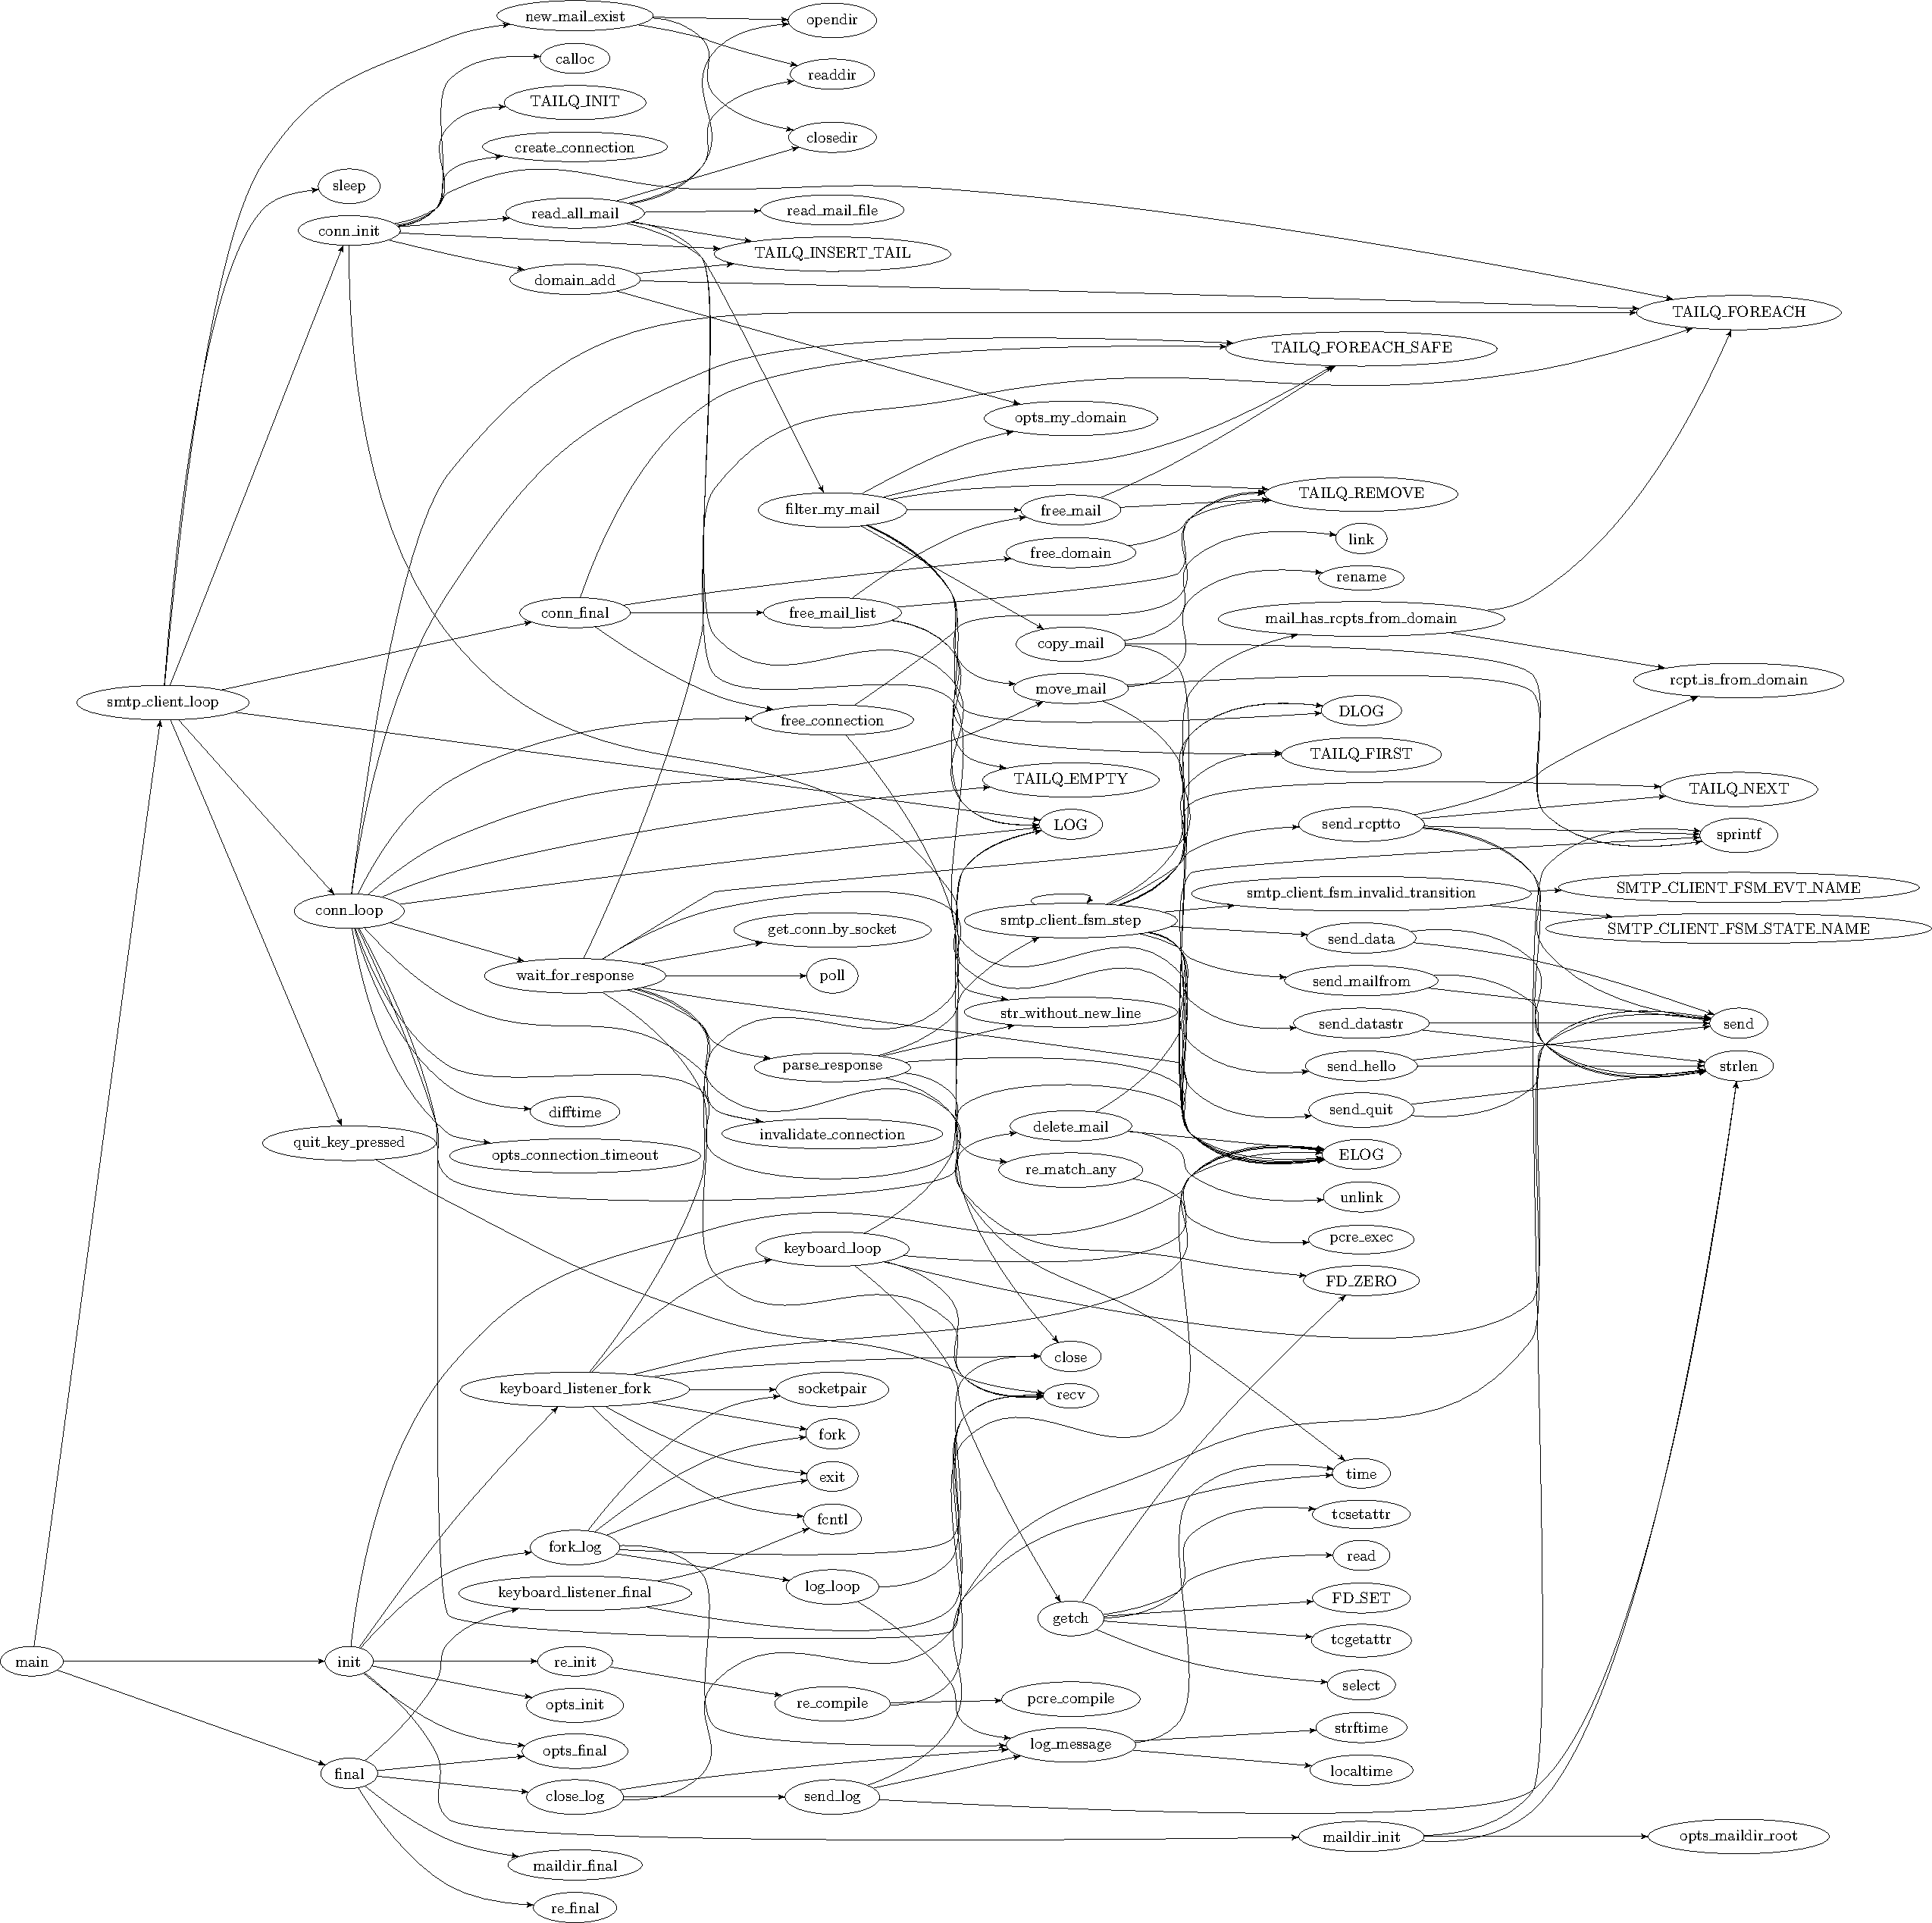
\includegraphics[width=\textwidth]{include/cflow01_dot.pdf}
\caption{Граф вызовов, основные функции}
\label{fig:cflow01}
\end{figure}

\begin{figure}
\centering
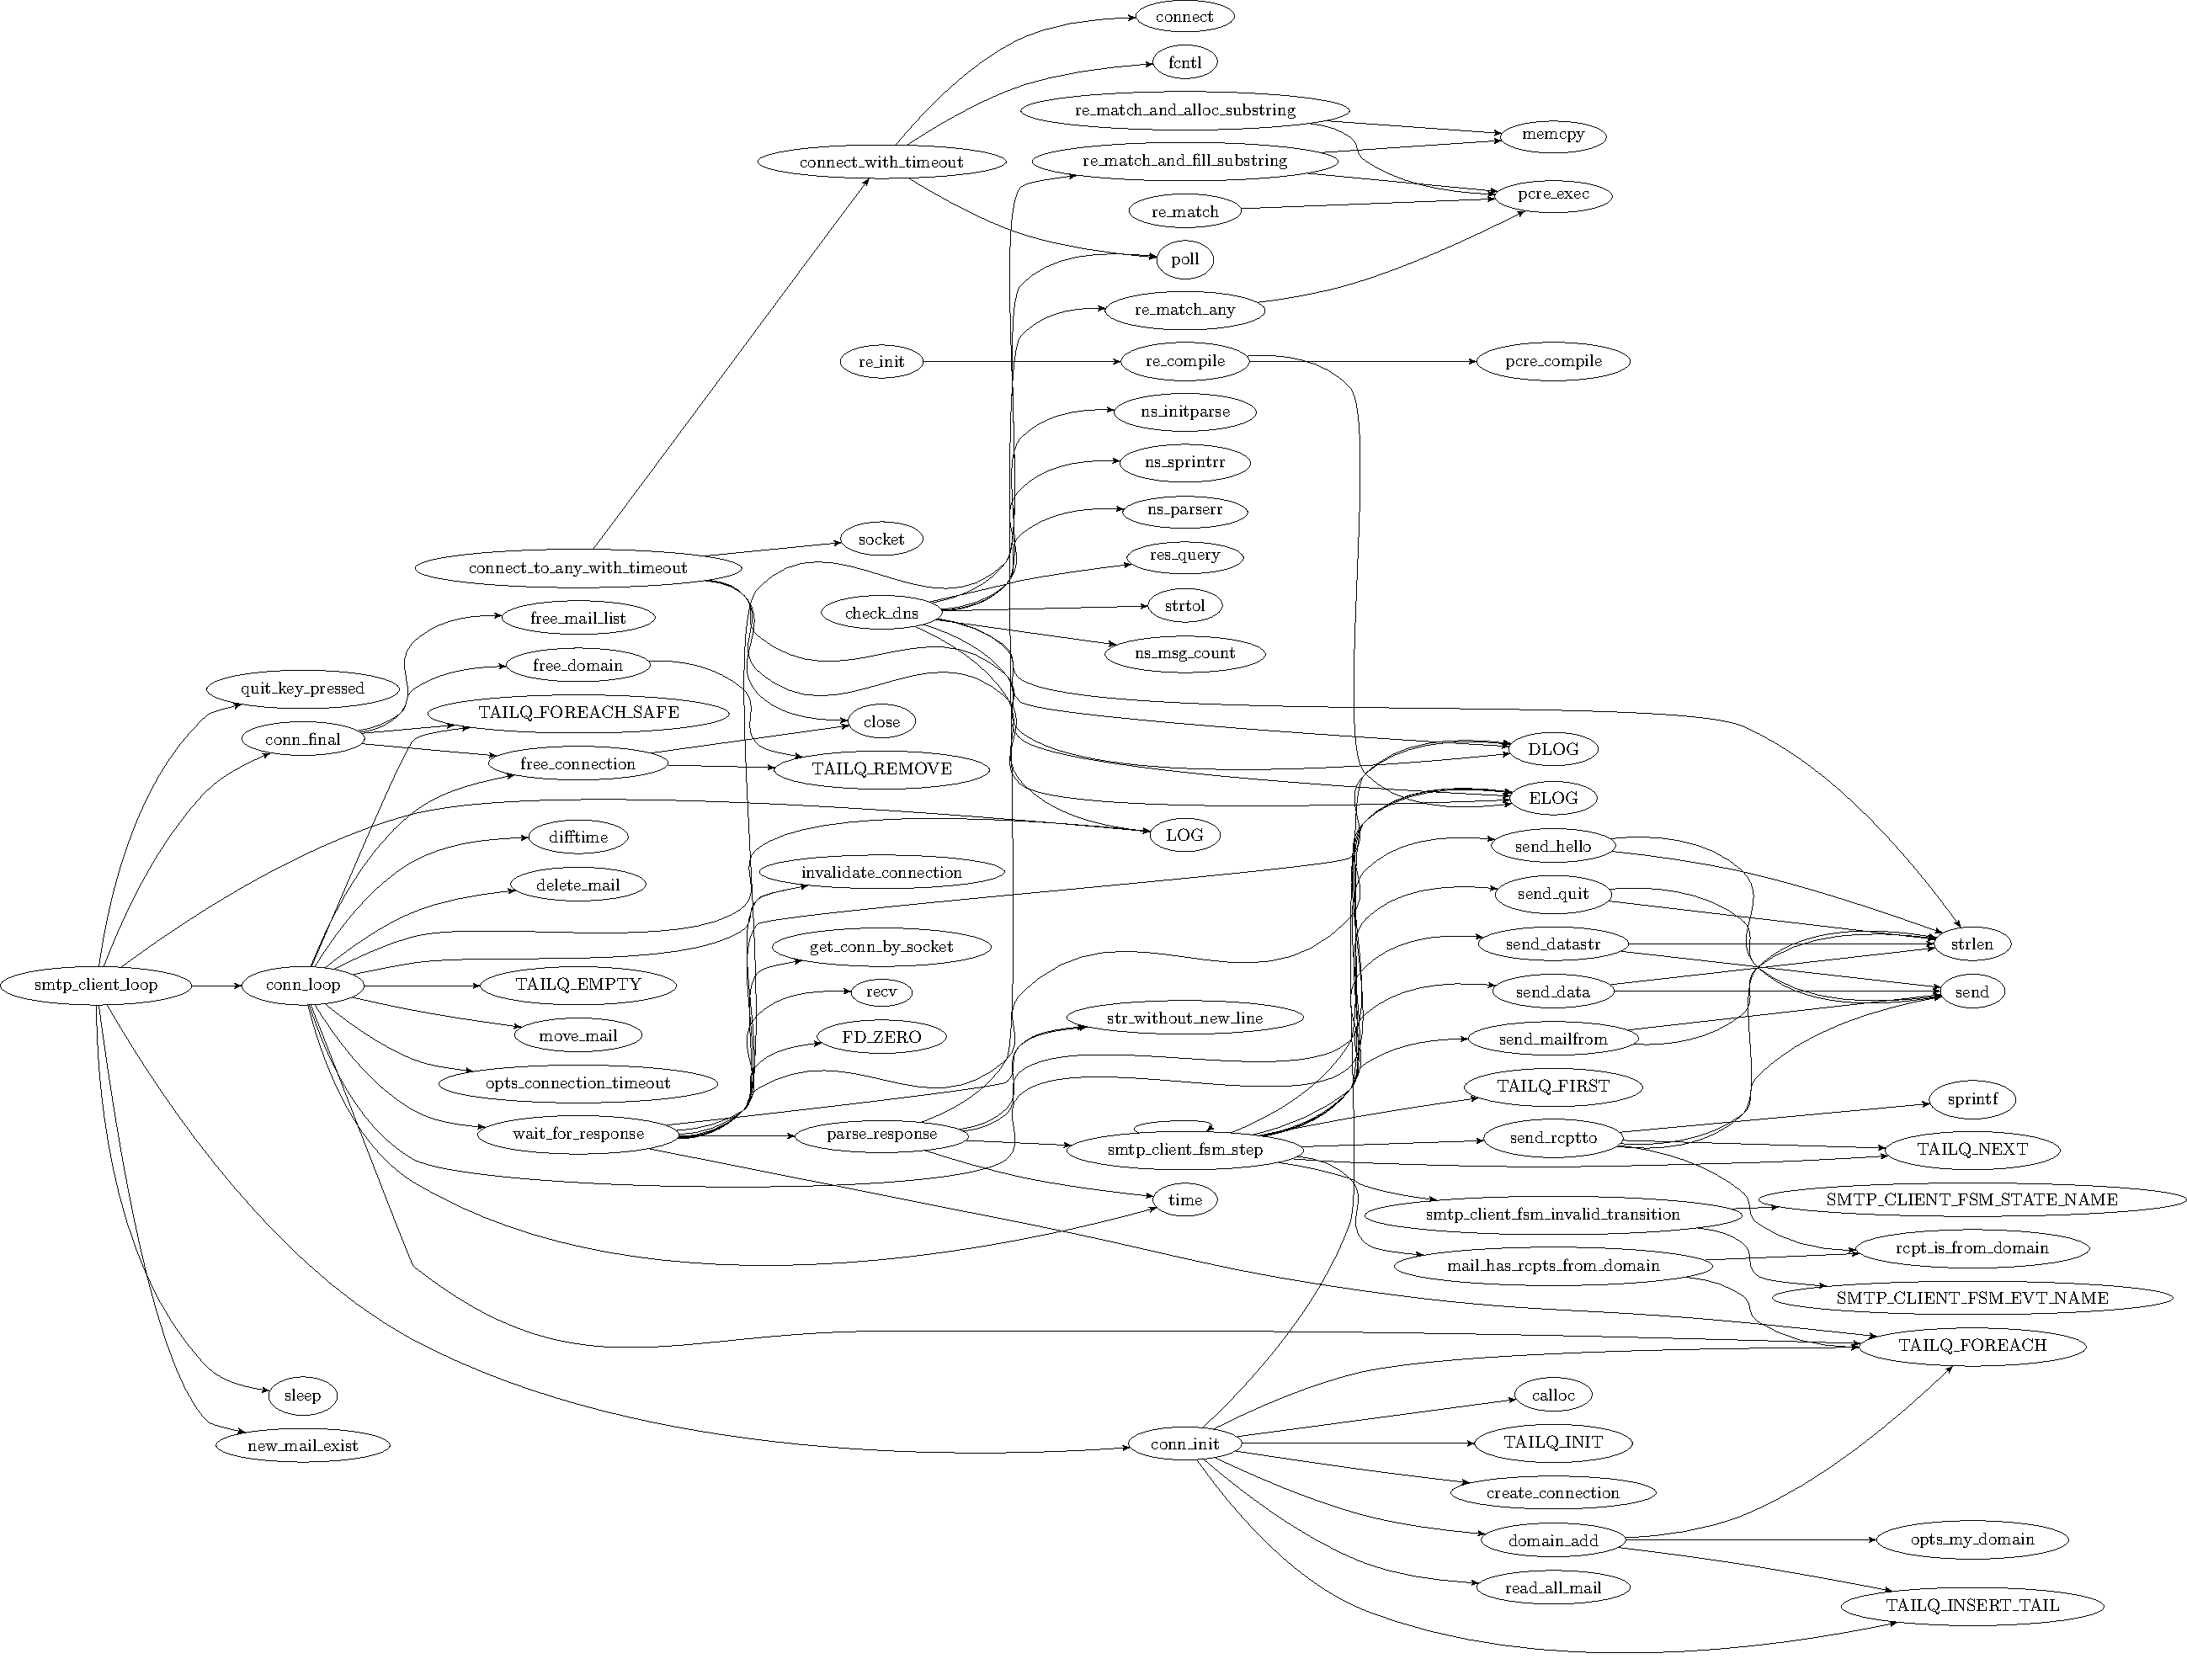
\includegraphics[width=\textwidth]{include/cflow02_dot.pdf}
\caption{Граф вызовов, функции обработки команд}
\label{fig:cflow02}
\end{figure}

Графы созданы с помощью \textit{cflow}, \textit{cflow2dot}, \textit{dot}.

\newpage
\section{ЗАКЛЮЧЕНИЕ}
Результатом данной работы является разработанная программа - SMTP-сервер, позволяющий производить получение электронной почты по протоколу SMTP. 

Также были решены все поставленные задачи: 

\begin{itemize}
		\item Реализован КА логики работы протокола SMTP клиента
		\item Создан алгоритм обработки нескольких соединений в рамках одного процесса с использованием вызова poll();
		\item Разработана программа - SMTP-клиент;
		\item Представлено описание реализованных функций программы, графа вызовов функций, процесса и графа сборки программы, реализованных алгоритмов для синхронизации доступа к данным;
		\item Проведенно модульное, системное тестирование, а также тестирование утечек памяти полученного SMTP-сервера. Выполнена оценка полученных результатов.

\end{itemize}

Использование вызова poll() позволило организовать обработку нескольких соединений в рамках одного рабочего процесса, а равномерное распределение подлючений между рабочими процессами позволило эффективно производить обслуживание множества подключений.

Программа Autogen с библиотеками AutoFSM и AutoOpts позволила быстро получить код КА для работы программы, а также функционал распознавания параметров командной строки.

По результатам проведенного модульного тестирования, с использования CUnit, а также системного тестирования были выявлены и устранены некоторые ошибки в функциях разработанной программы. А использование Valgrind позволило выявить и устранить места утечек памяти программы.

\end{document}
